%-----------------------
\chapter{Alkalmazás}
%-----------------------
%TODO write
%TODO spellcheck

Egy alkalmazás megvalósítása mindig komplex folyamat, mely sok kisebb részfolyamatot foglal magába. Az alábbiakban a fejlesztés részleteiről fogok írni, kezdve az alkalmazással szemben támasztott követelményekkel, majd képernyőképek segítségével bemutatom a működését. Ezután a megvalósítás részleteibe fogok belemenni, és végül a tesztelésről is ejtek pár szót.

\section{Követelmények}

A fejlesztés során alapvető célom volt egy, a modern paradigmáknak és a felhasználók elvárásainak megfelelő applikáció megalkotása. Törekedtem az objektumorientált szemlélet alkalmazására, a felelősségek szétválasztására és a maximális felhasználói élmény nyújtására. Fontos volt, hogy az alkalmazás folyamatai ne térjenek el nagymértékben attól, mint amit a felhasználók más applikációkban megszokhattak, és minden művelet meg legyen valósítva az adatokon, amire szükségük lehet. 

Ezek alapján az alábbi követelmények fogalmazódtak meg az alkalmazással szemben:
\begin{itemize}
	\item A felhasználónak legyen lehetősége fiókot létrehozni, e-mail cím és jelszó megadásával bejelentkezni, illetve fiókjából ki is lépni.
	\item Az adatok legyenek perzisztensen tárolva, az alkalmazás bezárásával, abból való kilépéssel vagy egy esetleges készülékcsere esetén sem veszhetnek el.
	\item Az adatok csak bejelentkezés után váljanak láthatóvá.
	\item A felhasználó képes legyen kategóriákat létrehozni a jegyzetek számára, ezeket akár tetszőleges mélységben más kategóriákba ágyazni.
	\item Legyen lehetőség jegyzetek létrehozására dokumentumok lefényképezése által. A digitalizált szöveg visszakapása után a jegyzet lehessen címmel ellátható, kategóriába sorolható és a tartalma szerkeszthető.
	\item Inkonzisztens adatok létrehozására ne adjon lehetőséget, a felhasználói input mindig legyen validálva.
	\item A jegyzeteken és kategóriákon lehessen minden fő műveletet - létrehozás, olvasás, módosítás, törlés - elvégezni, ezek során a felhasználói felület és az adatbázis maradjanak konzisztensek egymással.
	\item Módosítás során lehessen a jegyzetet újabb fényképek készítésével kiegészíteni, az ily módon digitalizált szöveg kerüljön hozzáfűzésre az eredeti tartalomhoz.
	\item A UI esztétikai és felhasználói élmény szempontjából legyen megfelelő, a hosszú ideig tartó folyamatokat jelezze a felhasználónak töltőképernyő segítségével. 
	\item A jegyzetek listája lehessen rendezhető és kereshető. 
\end{itemize}

\section{Működés}

\subsection{Bejelentkezés}
A telepítést követően a bejelentkezési képernyő az első, amivel a felhasználó találkozik. Ez már korábban megjelent a dolgozatban, a \refstruc{fig:MaterialBeforeAfter} bemutatásában. Itt a beviteli mezők segédszövegei egyértelműsítik, hogy milyen adatok elvártak a bejelentkezéshez illetve regisztrációhoz. Ezek gombnyomás hatására validálásra kerülnek, és amennyiben az e-mail formátuma nem érvényes vagy a jelszó hossza nem éri el a 6 karaktert, akkor a folyamat meghiúsul, és a felhasználó értesül róla, hogy mely mező(k) tartalmát kell javítania. 
%TODO picture if short on pages

\subsection{Kategorizált lista}
Sikeres bejelentkezést követően az alkalmazás a fő képernyőjére navigál, ahol az eddig elmentett jegyzeteket láthatjuk kategóriákba rendezve. A kategóriák alapértelmezetten össze vannak csukva, csak a legfelső szinten található elemeket látjuk. A lista sorainak jobb szélén elhelyezkedő nyilakra kattintva tudjuk kibontani az adott kategóriát, ezzel megtekinteni a tartalmát (\refstruc{fig:NoteListScreen}).

\begin{figure}[!ht]
	\centering
	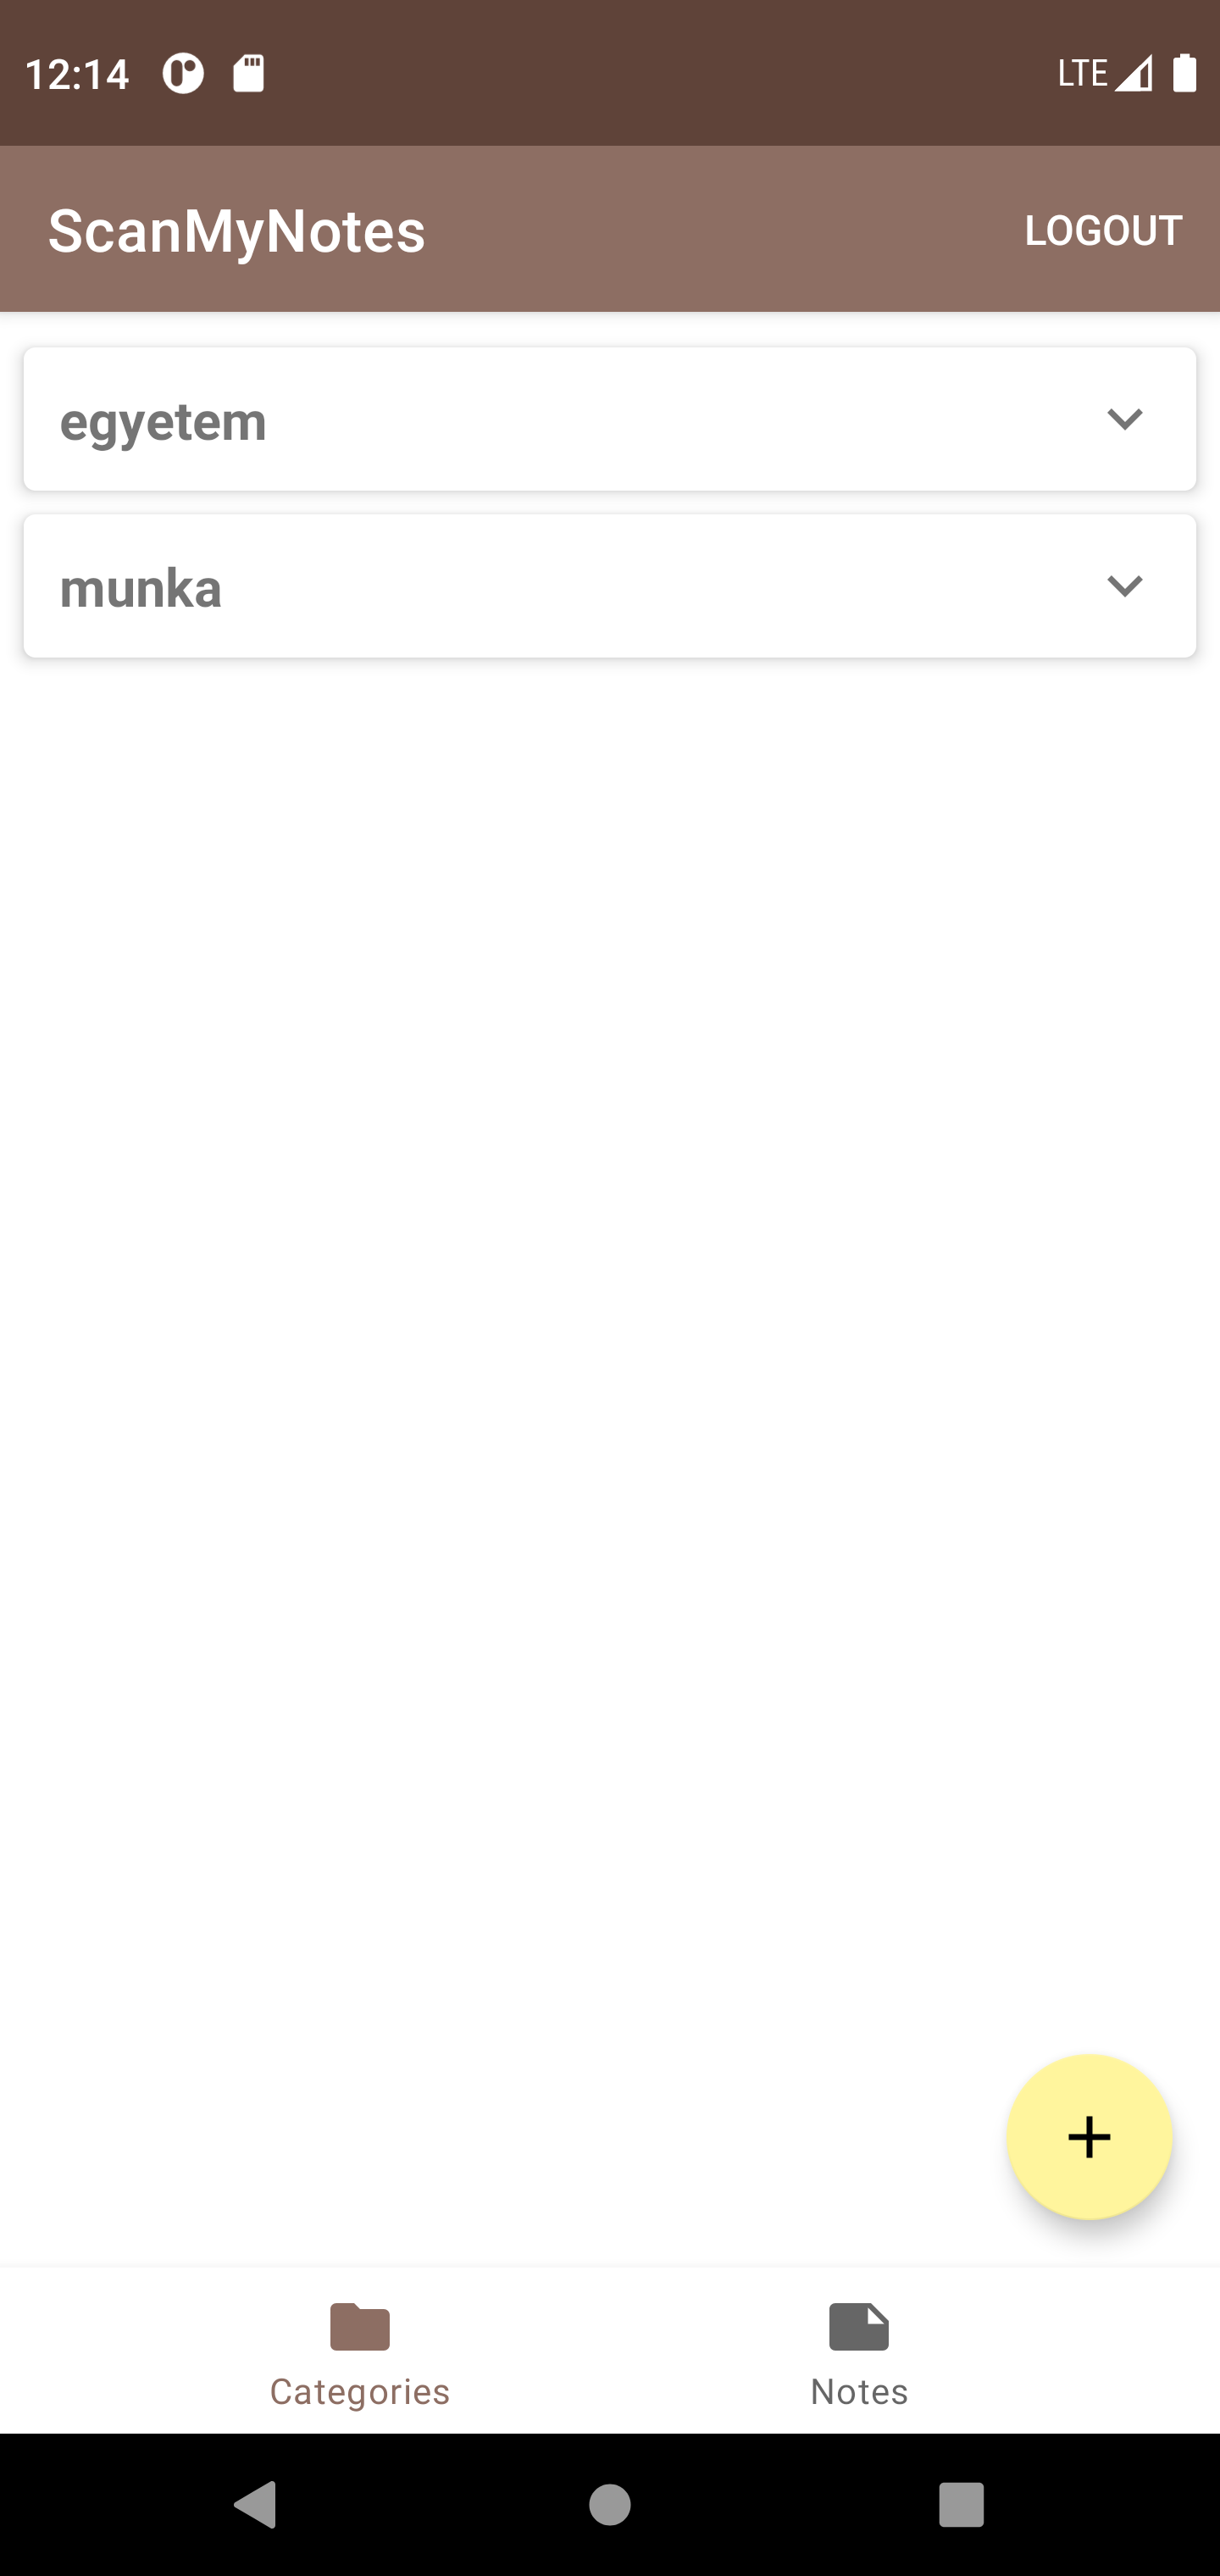
\includegraphics[width=60mm, keepaspectratio]{figures/notelist_closed.png}
	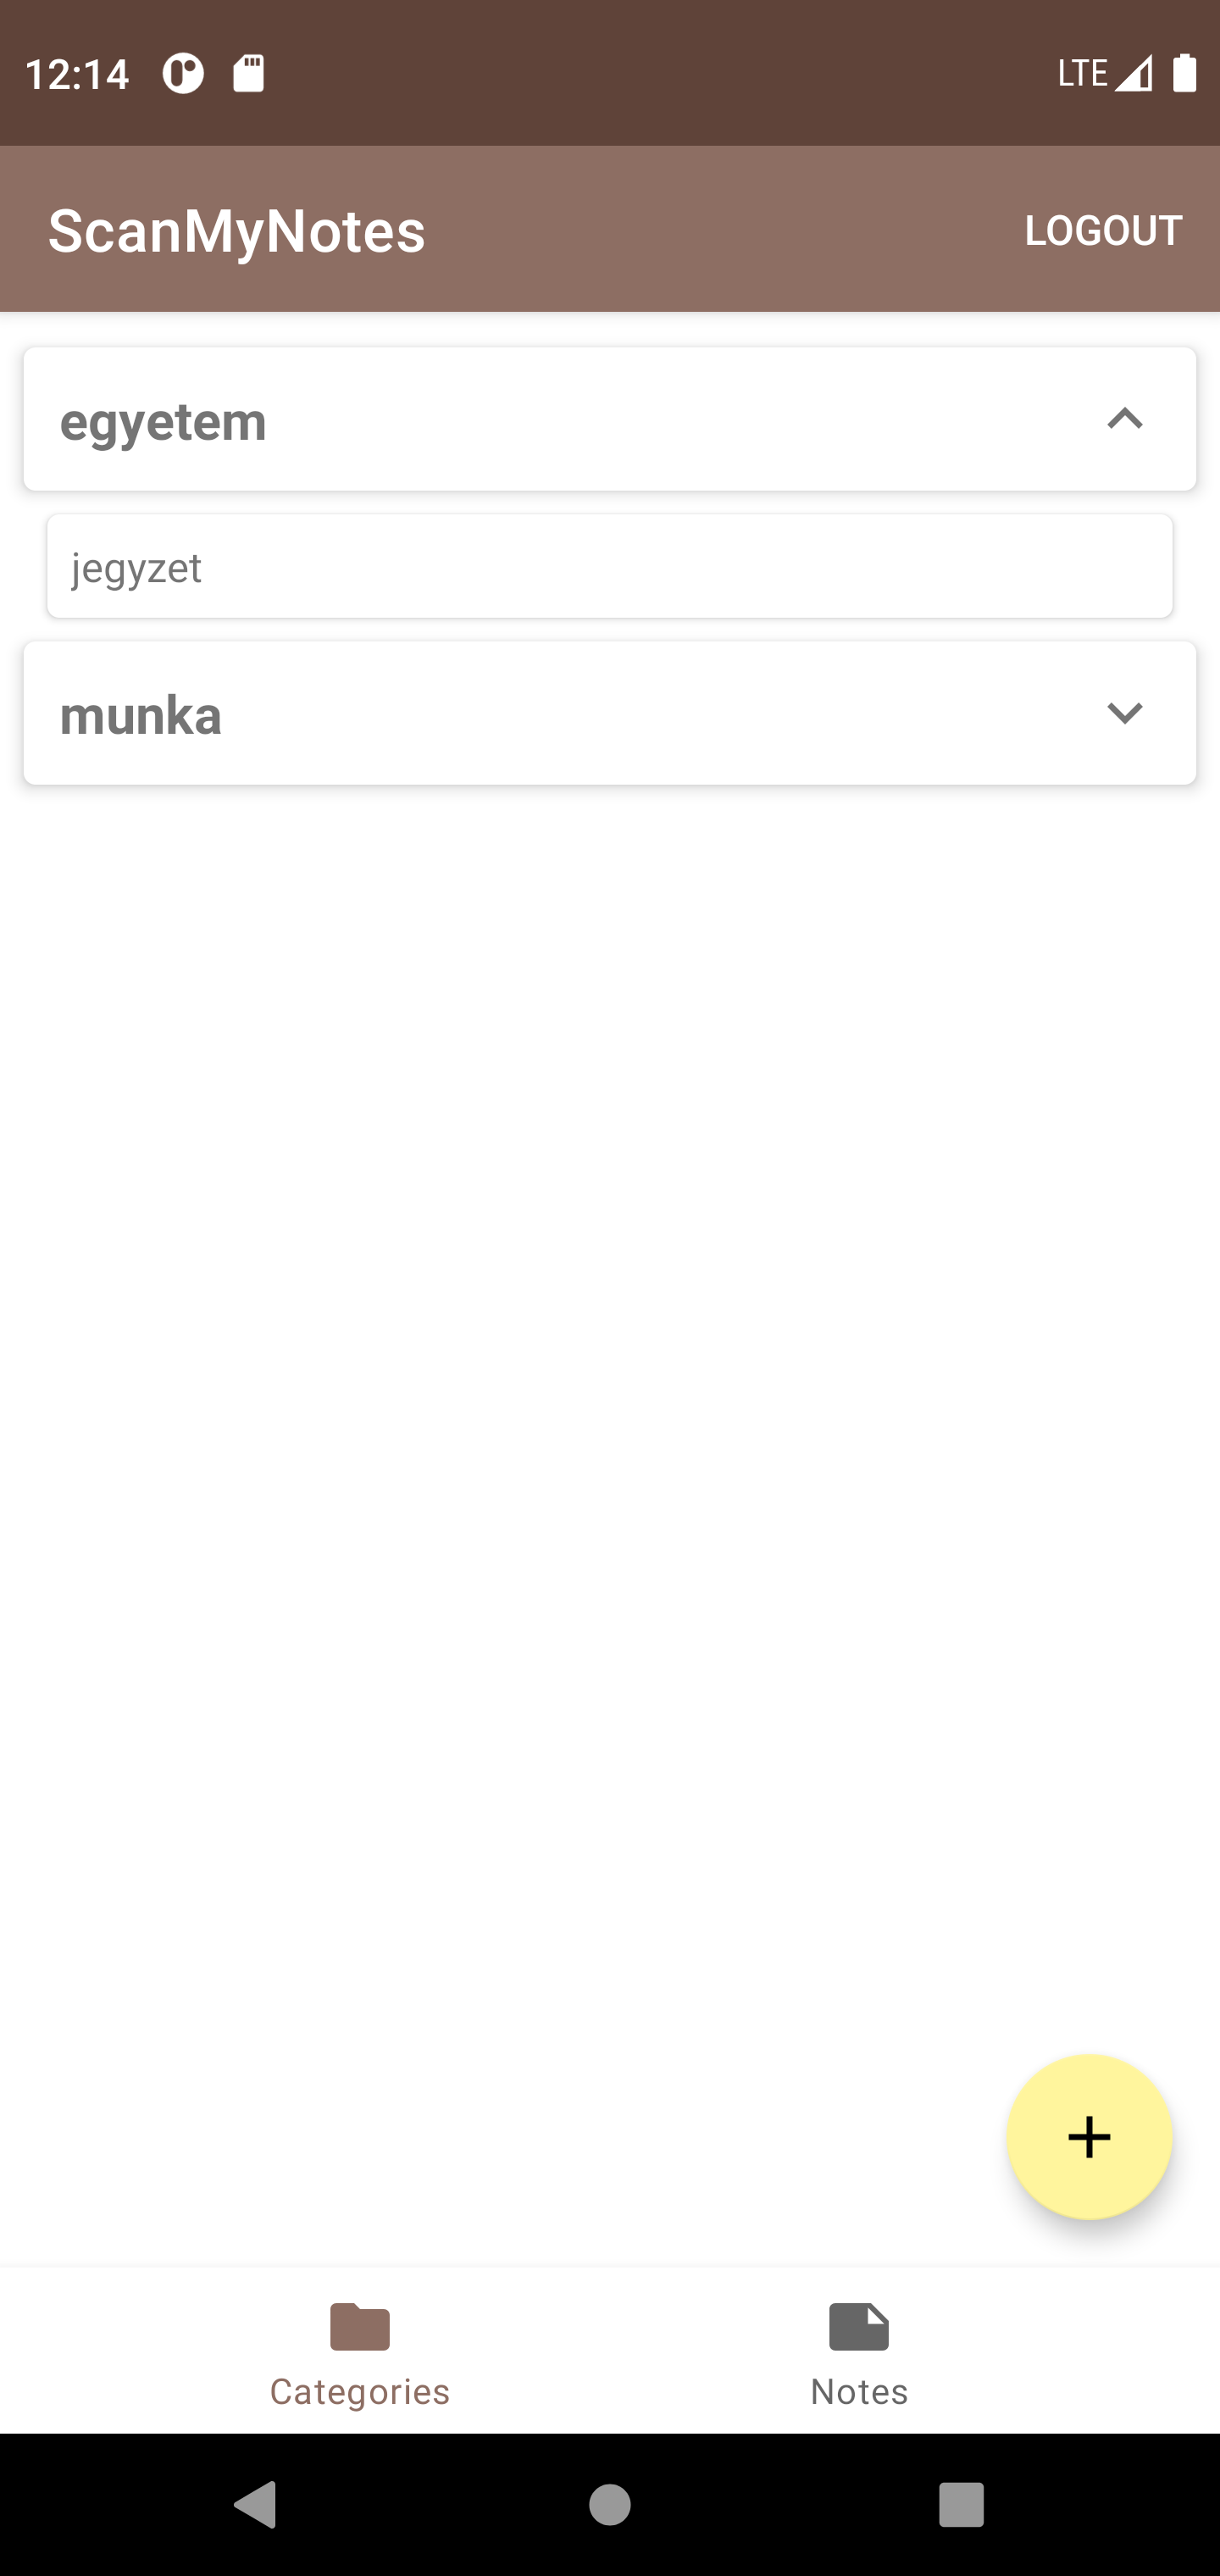
\includegraphics[width=60mm, keepaspectratio]{figures/notelist_open.png}
	\caption{Az alkalmazás kezdőlapja alapértelmezett állapotban, illetve egy kategória kibontva.}
	\label{fig:NoteListScreen}
\end{figure}

Innen számos lehetőségünk adódik navigációra az applikáción belül, kezdve a jobb felső sarokban található, meglehetősen magától értetődő kijelentkezés gombbal. Ezt megnyomva a fent leírt bejelentkezési képernyőre navigálunk, ahol adataink megadásával újra bejelentkezhetünk.

\subsection{Jegyzetlista}
A főképernyőn alul egy navigációs sávot találunk, mellyel a két különböző listamegjelenítés között tudunk váltani. Míg a \emph{Categories} opció alatt egy hierarchikusan egymás alá rendezett elemek listáját láthattuk, a \emph{Notes} opció csak a jegyzeteket tárja elénk, kategóriától függetlenül.  
%TODO kép - több jegyzetet felvenni hozzá
\section{Megvalósítás}

Ahogy az az ábrán is látható, nincs külön képernyő a bejelentkezés illetve a regisztráció lebonyolítására. Ez a döntés azért született meg, mert az alkalmazás jelenlegi funkcionalitásában nincs szerepe a felhasználói profilnak, nincs szükség semmilyen plusz információra a felhasználótól, ami később bármilyen formában felhasználásra kerülne. Így tökéletesen elegendő egyetlen képernyőn bekérni az adatokat az autentikációhoz, hiszen nem ad hozzá 

\section{Tesztelés}